% Shared preamble of the HSEMHS mode documents (docs/physics/*.tex, docs/technical/*.tex).
\documentclass[10pt]{extarticle}
\usepackage[a4paper,margin=1.7cm]{geometry}
\usepackage[T1]{fontenc}\usepackage{lmodern}\usepackage{tabularx}
\usepackage{amsmath,amssymb,bm,enumitem,titlesec,xcolor,booktabs,array,tikz,graphicx,longtable}
\usepackage[hidelinks]{hyperref}
\titleformat{\section}{\large\bfseries\color{blue!50!black}}{\thesection.}{0.5em}{}
\titlespacing*{\section}{0pt}{9pt}{3pt}
\titleformat{\subsection}{\normalsize\bfseries}{\thesubsection}{0.5em}{}
\titlespacing*{\subsection}{0pt}{6pt}{2pt}
\setlist{nosep,leftmargin=1.3em}
\setlength{\parindent}{0pt}\setlength{\parskip}{4pt}
\renewcommand{\arraystretch}{1.15}
\newcommand{\B}{\mathbf B}\newcommand{\J}{\mathbf J}\newcommand{\F}{\mathbf F}\newcommand{\R}{\mathbf R}
\newcommand{\zh}{\hat{\mathbf z}}\newcommand{\Bo}{\mathbf B_{\rm obs}}\newcommand{\Lv}{\mathbf L}
\newcommand{\code}[1]{\texttt{#1}}
\newcolumntype{L}[1]{>{\raggedright\arraybackslash}p{#1}}
\newcolumntype{Y}{>{\raggedright\arraybackslash}X}
\newcommand{\doctitle}[2]{{\Large\bfseries #1}\\[2pt]{\small #2}\par\vspace{2pt}}
\pagestyle{plain}
\AtBeginDocument{\sloppy}

\begin{document}
\doctitle{Where to stop the magnetohydrostatic solve on an optical-depth grid}{An experiment on the \code{logtau\_cut}
parameter of \code{mhs-poisson-ltau} in HSEMHS, tested against a Bifrost simulation. 26 October 2026.}

\begin{abstract}
\noindent The mode \code{mhs-poisson-ltau} computes gas pressure and geometric heights on optical-depth surfaces such that
pressure, gravity and the Lorentz force balance. It solves only the levels below a cut, $\log_{10}\tau_{500}\ge-4$ by
default, and keeps the layers above it in column hydrostatic equilibrium. The value $-4$ had been chosen on physical grounds
but never tested. We ran the solver on a full $504\times504$ Bifrost-derived atmosphere with the cut at $-4$, $-5$, $-6$ and
with no cut, and compared each result with the simulation's own pressures and heights. The cut at $-4$ is the only one that
converges; it reduces the error of the $\tau_{500}=1$ surface from 85\,km (column hydrostatic start) to 27\,km and
reproduces the Wilson depression of magnetic elements ($-78$\,km against $-74$\,km in the simulation). A cut at $-5$ is
slightly worse and five times slower. Cuts at $-6$ and above put layers with plasma $\beta\ll1$ into the solve; the solver
then tries to balance a Lorentz force of 10--1000 times the weight of the gas with the gas pressure, and the $\tau=1$ surface
is displaced by 1--20\,Mm. We recommend keeping $\code{logtau\_cut}=-4$ and, more generally, placing the cut where the
median $\beta$ is still $\gtrsim10$.
\end{abstract}

\section{The problem}
A spectral-line inversion gives the temperature $T$ and the magnetic field $\B$ in each pixel as functions of the continuum
optical depth $\tau_{500}$, but not the gas pressure $P$ or the geometric height $z$ of each optical-depth surface. HSEMHS
offers two ways to supply them on the $\tau$ grid:
\begin{itemize}
\item \code{column-hse-ltau}: every pixel column is put into hydrostatic equilibrium on its own,
$\mathrm d\ln P/\mathrm d\ln\tau = g\tau\rho/(\chi P)$ and $\mathrm dz/\mathrm d\ln\tau=-\tau/\chi$, with $\chi$ the
500\,nm extinction coefficient. Columns are not in horizontal balance with each other, and $\J\times\B$ is ignored.
\item \code{mhs-poisson-ltau}: starting from the column solution, a Gauss--Newton (Levenberg--Marquardt) solve looks for
$\ln P$ on the $\tau$ levels and the heights of the $\tau$ surfaces such that
\begin{equation}
-\nabla P - \rho g\,\zh + \J\times\B = 0,\qquad \J=\nabla\times\B/\mu_0,
\end{equation}
holds as well as possible in all three directions (weighted least squares), with $T$ and $\B$ held fixed.
\end{itemize}
The second mode does not solve all levels. Levels above a \emph{cut} $\log_{10}\tau<\code{logtau\_cut}$ are kept at the
column hydrostatic solution (their pressures and their distances to the cut level are fixed); only $\ln P$ below the cut and
one height per column are unknowns. The default $\code{logtau\_cut}=-4$ was set when the solver was written, by analogy
with the height-grid mode, where the solve is limited to $z\le1$\,Mm because solving into the upper atmosphere with a fixed
field inflated the pressure by 1--3 orders of magnitude. The specific value $-4$ had not been tested.

\textbf{Why a cut is needed at all.} The ratio of gas to magnetic pressure, $\beta=2\mu_0P/B^2$, falls steeply with height.
Where $\beta\ll1$ the Lorentz force of any field that is not force-free is much larger than the weight of the gas, and the
gas pressure cannot balance it. The field from an inversion (or from a dynamic simulation) is never force-free. If such a
layer is inside the solved region, the least-squares solve will still try to reduce that imbalance by changing the pressure.
On a $\tau$ grid this has a second effect: the height spacing of the levels, $\Delta z=-\int\tau/\chi\,\mathrm d\ln\tau$,
depends on the pressure through $\chi(T,P)$, and every height below a level is the sum of the spacings above it. A pressure
change high up therefore moves the whole column underneath, including the $\tau=1$ surface.

\textbf{Question.} Is $-4$ a good cut? What happens at $-5$, $-6$, and with no cut at all, and what physical quantity
should decide where the cut goes?

\section{Data and reference truth}
\textbf{Input.} \code{IO/input-mhs-ltau.nc}: $T$, $\B$ on 95 levels $\log_{10}\tau_{500}=-8.0,-7.9,\dots,1.4$ in
$504\times504$ columns. The file carries no $x,y$ axes; they were taken from the Bifrost cube it was made from (uniform
spacing $47.62$\,km, periodic). Gravity $g=274\,\mathrm{m\,s^{-2}}$; EOS and opacity from \code{cache/eos\_table\_fullz.h5}.

\textbf{Truth.} The input was derived from the Bifrost enhanced-network simulation \code{en024048\_hion}, snapshot 385,
which also holds the true $P$, $\rho$ and $z$. We computed $\tau_{500}$ for every Bifrost column from its own $T$ and $P$
with the same opacity table (top-first trapezoid, as the code does), and interpolated $z$, $\ln P$, $\ln\rho$, $\ln T$
linearly in $\log\tau$ onto the 95 input levels. As a check, the input temperature agrees with the interpolated Bifrost
temperature to 0.1--1\,\% (median) between $\log\tau=-4.5$ and $-0.5$, and to 1--9\,\% higher up. Individual points can
differ by much more (up to a factor $\sim$2), so the input's $\tau$ scale was built with a somewhat different opacity or
interpolation. \emph{The truth is therefore reliable for statistics over many points, not point by point.} All heights are
compared after removing the mean of $z(\tau=1)$ (the code's own gauge).

\section{Experiments}
Five runs of the production code (main at \code{5e901b5}), identical except for the cut:

\begin{center}\small
\begin{tabular}{llll}
\toprule
run & mode & \code{logtau\_cut} & solved $\ln P$ levels per column\\
\midrule
column HSE & \code{column-hse-ltau} & -- & none (reference start)\\
cut $-4$ & \code{mhs-poisson-ltau} & $-4.0$ (default) & 54\\
cut $-5$ & \code{mhs-poisson-ltau} & $-5.0$ & 64\\
cut $-6$ & \code{mhs-poisson-ltau} & $-6.0$ & 74\\
no cut & \code{mhs-poisson-ltau} & $-7.9$ (top level, the highest allowed) & 93\\
\bottomrule
\end{tabular}
\end{center}
All other settings are the defaults: alignment of the starting columns on total pressure $P+B^2/2\mu_0$, at most 100 steps,
stop when the relative decrease of the objective $\Phi$ is below $10^{-4}$ on three consecutive steps, height step cap
300\,km. Each run used one hyades node (3--4 MPI ranks $\times$ 32--48 threads).

\section{What we measured}
\begin{enumerate}
\item \textbf{Convergence:} number of steps, stop reason, $\Phi/\Phi_0$, the Gauss--Newton decrement (relative decrease a
further full step would give; small means stationary), wall time.
\item \textbf{Accuracy against Bifrost:} rms and median of $\ln(P/P_{\rm Bifrost})$ and rms of $z-z_{\rm Bifrost}$ on each
level, for all columns and separately for strong-field ($|\B|>500$\,G at $\tau=1$; 1.2\,\% of columns) and quiet
($<100$\,G; 91.5\,\%) columns.
\item \textbf{The $\tau=1$ surface:} map of $z(\tau=1)$, its rms error and correlation with Bifrost, and the \emph{Wilson
depression}, the mean $z(\tau=1)$ of strong-field minus quiet columns. Magnetic elements are evacuated, so their $\tau=1$
surface lies deeper; in this snapshot by $74$\,km.
\item \textbf{Pressure inflation:} $\ln(P/P_{\rm column\,HSE})$ on the solved levels, i.e. how far the solve moves the
pressure from the hydrostatic start.
\item \textbf{Force balance, the same for every state:} independent of the solver's own residuals and weights, we evaluate
on every point the net force over the weight of the gas,
\begin{equation}
\frac{\F_h}{\rho g}=H\Bigl(-\nabla_h\ln P\big|_z+\frac{\Lv_h}{P}\Bigr),\qquad
\frac{F_z}{\rho g}=H\Bigl(-\partial_z\ln P-\frac{\rho g}{P}+\frac{L_z}{P}\Bigr),\qquad H=\frac{P}{\rho g},
\end{equation}
with $\Lv=\J\times\B$, horizontal derivatives at fixed height and centred differences. Applied to the Bifrost truth this gives
the imbalance a real, dynamic atmosphere has (Bifrost has flows, so it is not static).
\item \textbf{Plasma $\beta$ and $|\Lv|/\rho g$} per level (from Bifrost), the scale of what the field can do compared with
gravity.
\end{enumerate}

\section{Results}
\subsection{Summary}
\begin{center}\small
\begin{tabular}{lrlrrrrr}
\toprule
run & steps & stop & $\Phi/\Phi_0$ & wall & $z(\tau{=}1)$ err (rms) & corr. & Wilson depr.\\
\midrule
column HSE & -- & -- & -- & 1.3 min & 85 km & 0.61 & $-106$ km\\
\textbf{cut $-4$} & 19 & converged & $1.8\times10^{-2}$ & 16 min & \textbf{27 km} & \textbf{0.69} & $\mathbf{-78}$ \textbf{km}\\
cut $-5$ & 100 & max\_steps & $2.2\times10^{-3}$ & 89 min & 40 km & 0.62 & $-104$ km\\
cut $-6$ & 100 & max\_steps & $1.1\times10^{-1}$ & 64 min & 1\,137 km & 0.09 & $-180$ km\\
no cut & 100 & max\_steps & $1.8\times10^{-1}$ & 81 min & 20\,184 km & 0.06 & $-16$ Mm\\
Bifrost & & & & & 0 & 1 & $-74$ km\\
\bottomrule
\end{tabular}
\end{center}
$\Phi_0$ itself grows by fifteen orders of magnitude as the cut moves up ($7.4\times10^{10}$, $1.2\times10^{13}$,
$3.1\times10^{17}$, $2.9\times10^{25}$ for $-4,-5,-6$, none): the objective is increasingly dominated by the force
imbalance of the upper layers. Ratios $\Phi/\Phi_0$ are therefore not comparable between runs.

\subsection{Where the field takes over}
\begin{center}\small
\begin{tabular}{rrrr|rrrrrr}
\toprule
 & \multicolumn{3}{c|}{Bifrost} & \multicolumn{6}{c}{median $|\F_h|/\rho g$}\\
$\log\tau$ & median $\beta$ & frac.\ $\beta<1$ & $|\Lv|/\rho g$ & Bifrost & col.\ HSE & cut $-4$ & cut $-5$ & cut $-6$ & no cut\\
\midrule
$-6.0$ & 0.014 & 0.98 & 14.6 & 11.1 & 8.6 & 8.0 & 8.0 & 8.4 & 21.5\\
$-5.5$ & 0.15 & 0.73 & 2.9 & 2.1 & 0.64 & 0.35 & 0.37 & 1.8 & 5.6\\
$-5.0$ & 3.0 & 0.35 & 0.18 & 0.21 & 0.36 & 0.14 & 0.14 & 1.3 & 4.4\\
$-4.5$ & 10.7 & 0.13 & 0.080 & 0.10 & 0.29 & 0.088 & 0.068 & 1.2 & 4.2\\
$-4.0$ & 21 & 0.05 & 0.050 & 0.073 & 0.27 & 0.049 & 0.056 & 1.1 & 4.1\\
$-3.0$ & 162 & 0.017 & 0.013 & 0.054 & 0.24 & 0.021 & 0.047 & 1.1 & 4.1\\
$-2.0$ & 4\,200 & 0.005 & 0.0006 & 0.055 & 0.23 & 0.018 & 0.045 & 1.1 & 4.1\\
$-1.0$ & 17\,900 & 0.002 & 0.0001 & 0.071 & 0.21 & 0.027 & 0.054 & 1.1 & 4.1\\
$0.0$ & 23\,200 & 0.001 & 0.0001 & 0.098 & 0.15 & 0.045 & 0.065 & 1.0 & 4.1\\
\bottomrule
\end{tabular}
\end{center}
The median $\beta$ crosses 1 at $\log\tau\approx-5.5$. At $-4$ the gas dominates almost everywhere ($\beta\approx21$, 5\,\%
of points below 1, Lorentz force 5\,\% of the weight). At $-5$ a third of the points already have $\beta<1$; above $-6$
practically all do and the Lorentz force is 15--350 times the weight.

\begin{figure}[h]
\centering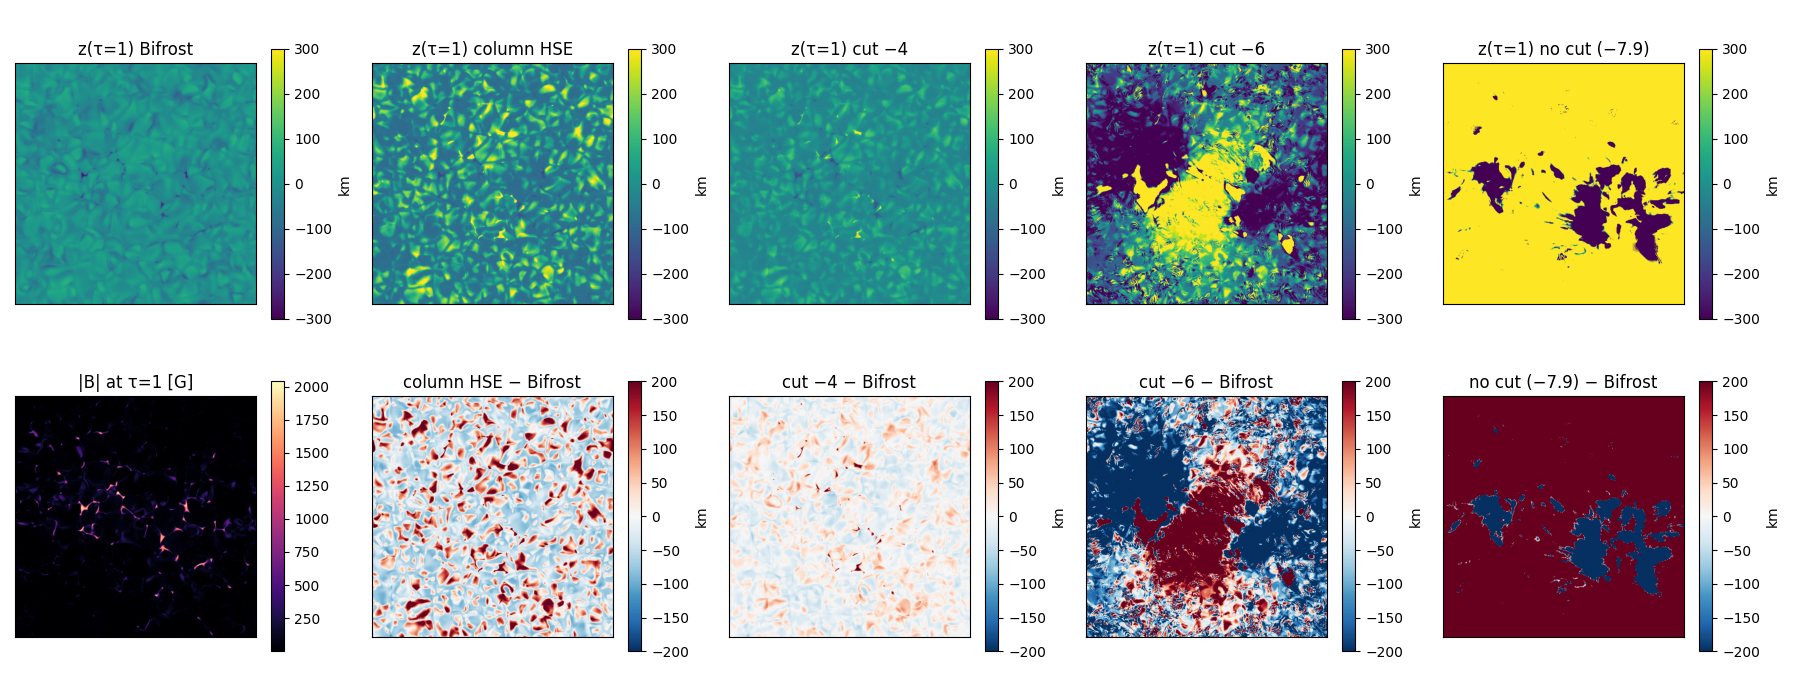
\includegraphics[width=\textwidth]{ztau1.png}
\caption{Top: height of the $\tau_{500}=1$ surface (each map's mean removed) in Bifrost, column HSE, and the cut $-4$, $-6$
and no-cut solutions; bottom left: $|\B|$ at $\tau=1$; bottom: difference from Bifrost. Colour ranges $\pm300$\,km (top)
and $\pm200$\,km (bottom) saturate for cut $-6$ and no cut.}
\label{fig:z1}
\end{figure}

\subsection{The \texorpdfstring{$\tau=1$}{tau=1} surface (Fig.~\ref{fig:z1})}
Column HSE gives the granulation pattern with exaggerated contrast: every column is hydrostatic on its own and aligned
only through one total-pressure level, and many structures sit 100--200\,km too high or too low. The cut $-4$ solve removes most of
this: the remaining error is small and unstructured, the rms error drops threefold and the Wilson depression of the
magnetic elements comes out at $-78$\,km against $-74$\,km in Bifrost (column HSE: $-106$\,km). With the cut at $-6$ the
surface is pushed up and down by up to several Mm in patches tens of Mm across; with no cut nearly the whole surface is
shifted by Mm, the mean gauge then hiding a few deep regions (down to $-60$\,Mm at the 1st percentile).

\begin{figure}[t]
\centering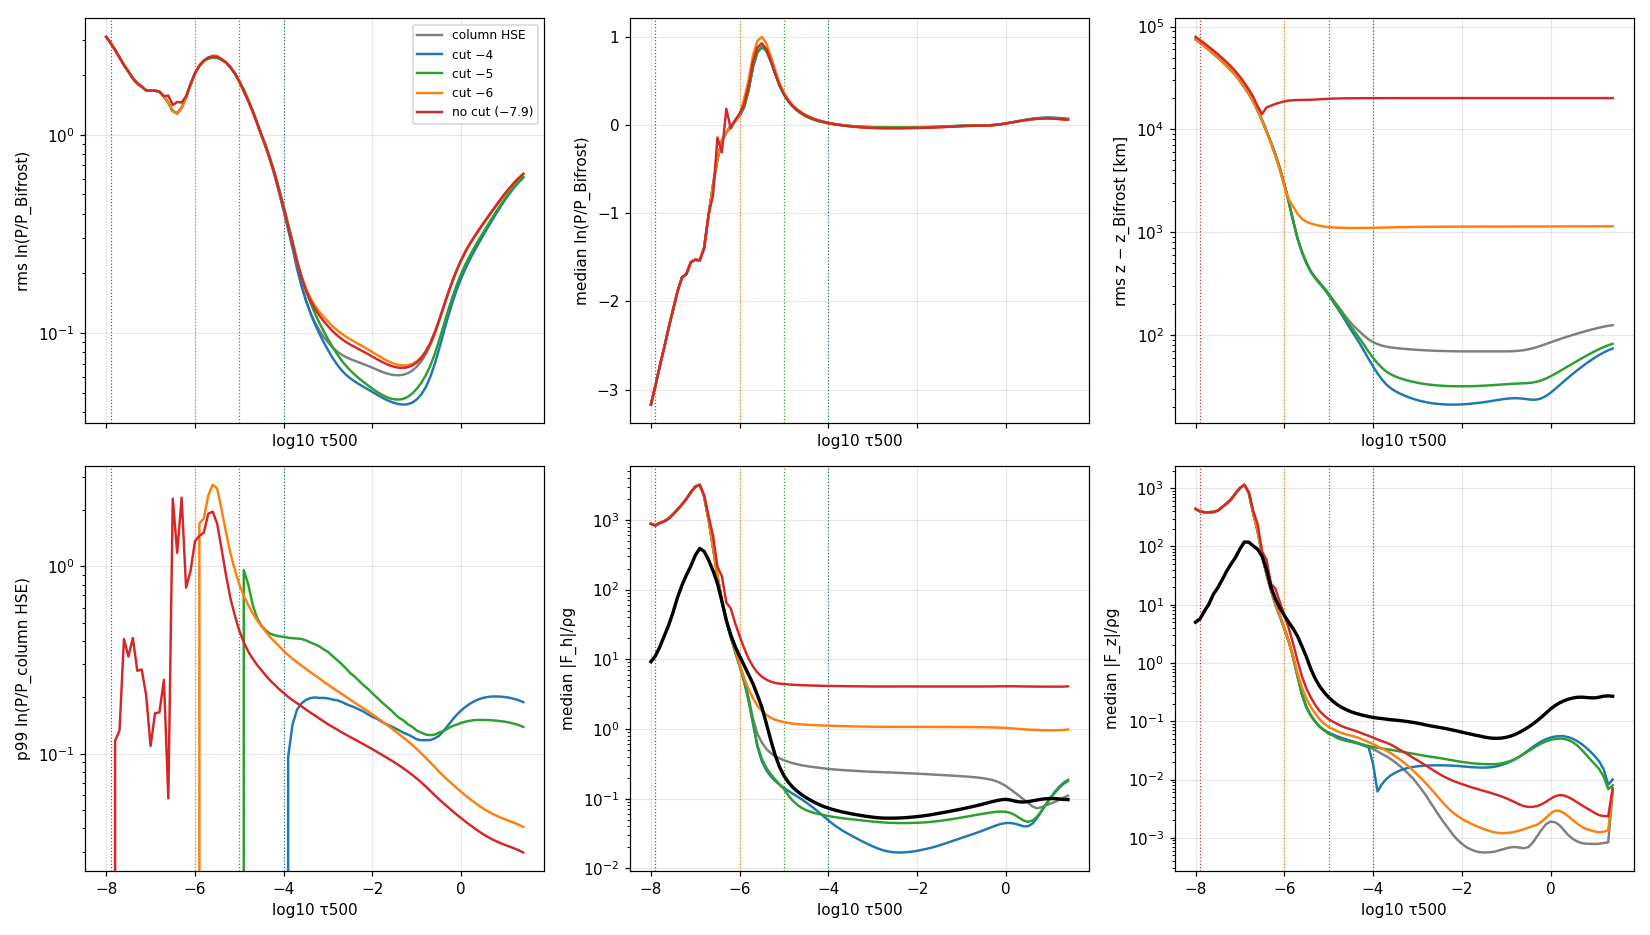
\includegraphics[width=\textwidth]{profiles.png}
\caption{Per-level statistics against $\log_{10}\tau_{500}$. Top: rms and median of $\ln(P/P_{\rm Bifrost})$; rms of
$z-z_{\rm Bifrost}$. Bottom: 99th percentile of $\ln(P/P_{\rm column\,HSE})$ (pressure inflation by the solve; zero above
each cut by construction); median net horizontal and vertical force over $\rho g$. Black: Bifrost. Dotted verticals: the
cut of the run with the same colour.}
\label{fig:prof}
\end{figure}

\subsection{Profiles (Fig.~\ref{fig:prof})}
\begin{itemize}
\item \textbf{Heights} (top right): between $\log\tau=-3$ and $0$ the height error is 20--30\,km for cut $-4$, 30--40\,km for
cut $-5$, 70\,km for column HSE (all rise below $\tau=1$), $\sim$1\,Mm for cut $-6$ and $\sim$20\,Mm for no cut. Because heights are sums of the
spacings above, an error made high in the column is carried unchanged to every level below: the curves are flat below the
layer where the damage happens.
\item \textbf{Pressure} (top left and middle): between $\log\tau=-3$ and $0$ cut $-4$ has the smallest rms error
(0.04--0.1, i.e.\ 4--10\,\%); all runs share the same large error above $-4$ (rms 1.5--3, a factor 5--20), because the
$\tau$-hydrostatic upper atmosphere does not describe Bifrost's dynamic chromosphere and transition region (the input
temperature also deviates most there). Near and below $\tau=1$ every run has errors of 0.3--0.6, which are equally present in
column HSE: they come from the $\tau$ scale mismatch and from Bifrost's convective pressure fluctuations, not from the cut.
\item \textbf{Inflation} (bottom left): the higher the cut, the more the solve raises the pressure just below it (99th
percentile up to $e^{2.7}\approx15$ times the hydrostatic value at the $-6$ cut).
\item \textbf{Force balance} (bottom middle and right): cut $-4$ and $-5$ bring the horizontal imbalance in the photosphere
from 0.2--0.3\,$\rho g$ (column HSE) to 0.02--0.06\,$\rho g$, which is \emph{below} Bifrost's own 0.05--0.1\,$\rho g$.
A static model should not be expected to do better than this. Cut $-6$ and no cut end at 1 and 4\,$\rho g$ everywhere below
the cut: worse than doing nothing.
\end{itemize}

\subsection{Error against \texorpdfstring{$\beta$}{beta}}
Figure~\ref{fig:beta} shows the distribution of $\ln(P/P_{\rm Bifrost})$ against the Bifrost $\beta$ for all points. At
$\beta>1$ the errors are concentrated around zero for all runs; the large errors are at $\beta<1$, i.e.\ in the fixed
upper part, and are inherited from the hydrostatic start. The point-wise pressure error is thus similar for all cuts; what
differs is the geometry (Fig.~\ref{fig:z1}), which is where a high cut does its damage.

\begin{figure}[h]
\centering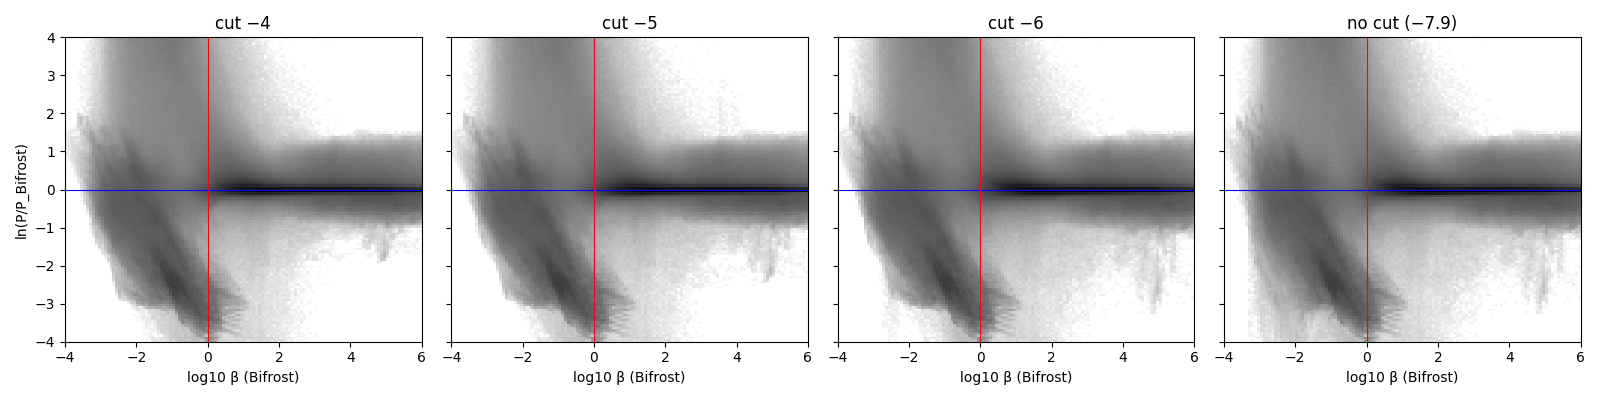
\includegraphics[width=\textwidth]{err_vs_beta.png}
\caption{Two-dimensional histogram (log counts) of $\ln(P/P_{\rm Bifrost})$ against $\log_{10}\beta$ (Bifrost), all levels and
columns. Red line: $\beta=1$.}
\label{fig:beta}
\end{figure}

\section{Interpretation}
\begin{enumerate}
\item \textbf{Why the high cuts fail.} The input field is not force-free (it comes from a dynamic simulation; an inverted
field will not be force-free either). In the layers with $\beta\ll1$ the residual Lorentz force is $10$--$1000\,\rho g$. A
least-squares solve with only the pressure free cannot remove it; it reduces it partially by large pressure changes. These
changes alter the opacity, hence the height spacing of the levels, and every height below moves with them. The objective
is dominated by these upper residuals (15 orders of magnitude in $\Phi_0$), so the solver accepts a much worse photosphere in
exchange for a small relative gain above. The step lengths stay tiny (line search $\alpha\approx0.02$ for no cut) and none of
these runs converge in 100 steps.
\item \textbf{Why $-4$ works.} Down to $\log\tau=-4$ the gas dominates ($\beta\approx20$, Lorentz force $\approx5$\,\% of the
weight), so the pressure can absorb the remaining imbalance with small changes, and the solved region contains the
photosphere where the inversion constrains $T$ and $\B$ best.
\item \textbf{Why $-5$ is not better.} It adds the layer where $\beta$ falls through 1--10 and 35\,\% of points are already
magnetically dominated. The solve still converges toward a reasonable state but slowly (not converged in 100 steps, 89\,min),
and those extra levels pull the $\tau=1$ heights of magnetic elements too deep (Wilson depression $-104$\,km).
\end{enumerate}

\section{Conclusions}
\begin{itemize}
\item Keep \code{logtau\_cut} $=-4$. It is the only cut tested that converges, it is the fastest of the solves, and it gives
the best heights ($z(\tau{=}1)$ error 27\,km, Wilson depression within 4\,km of the simulation) and a photosphere in better force
balance than the simulation itself.
\item The cut must lie in the gas-dominated layer. A practical rule: put it where the median $\beta$ of the starting state is
still $\gtrsim10$ and only a few percent of points have $\beta<1$. For a strongly magnetised field of view (sunspots, plage)
this level lies deeper and the cut should be moved down accordingly; for this enhanced-network snapshot it is
$\log\tau\approx-4$.
\item Solving without a cut, or with the cut in the low-$\beta$ layer, is harmful: the pressure absorbs an unbalanceable
Lorentz force and displaces the whole $\tau=1$ surface by Mm.
\item The pressure above the cut is not reliable in any run (off by a factor 5--20 against Bifrost): hydrostatic equilibrium
in $\tau$ does not describe a dynamic chromosphere. Results above $\log\tau\approx-4$ should not be interpreted as physical
pressures.
\end{itemize}

\textbf{Limitations.} One snapshot of one simulation (enhanced network, weak fields: 1.2\,\% of columns above 500\,G at
$\tau=1$); cuts tested only at whole decades; the reference truth on the $\tau$ grid is only statistically consistent with
the input (Sect.~2). A sunspot or plage field of view, and a $\beta$-based automatic cut, would be the natural next tests.

\textbf{Reproduction.} Branch \code{ltau-cut-study}: \code{HSEMHS/scripts/ltaucut/truth\_on\_tau.jl} (truth on the $\tau$
grid), \code{force\_diag.jl} (force balance), \code{analyse.py} (statistics and figures); configurations, logs and outputs in
\code{HSEMHS/out/ltaucut/} of the cluster worktree \code{MHS\_ltaucut}.
\end{document}
